%%%%%%%%%%%%%%%%%%%%%%%%%%%%%%%%%%%%%%%%%%%%%%%%%%%%%%%%%%%%%%%%%%
%
% Analysis of Algorithms
%
% Homework Assignment #3
%
%%%%%%%%%%%%%%%%%%%%%%%%%%%%%%%%%%%%%%%%%%%%%%%%%%%%%%%%%%%%%%%%%%
%%%%%%%%%%%%%%%%%%%%%%%%%%%%%%%%%%%%%%%%%%%%%%%%%%%%%%%%%%%%%%%%%%
%
% Score Card and Answer Sheets
%
%%%%%%%%%%%%%%%%%%%%%%%%%%%%%%%%%%%%%%%%%%%%%%%%%%%%%%%%%%%%%%%%%%
\documentclass[addpoints,11pt]{exam}
\usepackage{clrscode3e}
\usepackage{commath}
\usepackage{units}
\usepackage{enumitem}
\usepackage{fullpage}
\usepackage[usenames,dvipsnames]{xcolor}
\usepackage{amsmath}
\usepackage{amstext}
\usepackage{pdfpages}
\usepackage{tikz}
\usepackage{tikz-qtree}
\usepackage{booktabs}
\usepackage{float}

%%%%%%%%%%%%%%%%%%%%%%%%%%%%%%%%%%%%%%%%%%%%%%%%%%%%%%%%%%%%%%%%%%
%
% Begin Document
%
%%%%%%%%%%%%%%%%%%%%%%%%%%%%%%%%%%%%%%%%%%%%%%%%%%%%%%%%%%%%%%%%%%
\begin{document}
\pagestyle{empty}


\noindent{\large\bfseries Name: \hrulefill John Henry Mejia}\\
\noindent{\large\bfseries COSC 40403 - Analysis of Algorithms: Homework 3}\\
\noindent{\large\bfseries Due: 10:59:59 on September 27}

%%%%%%%%%%%%%%%%%%%%%%%%%%%%%%%%%%%%%%%%%%%%%%%%%%%%%%%%%%%%%%%%%%
%
% Score Card and Answer Sheets
%
% Comment out one-or-the-other to show or not-show the answers.
%
%%%%%%%%%%%%%%%%%%%%%%%%%%%%%%%%%%%%%%%%%%%%%%%%%%%%%%%%%%%%%%%%%%
%\SolutionEmphasis{\color{Blue}}
\renewcommand{\solutiontitle}{\noindent\textbf{Answer:}\par\noindent}
\printanswers
%%\noprintanswers


Some of the questions below require you to draw a graph or to trace through a graph algorithm.  Please use \LaTeX or another computer drawing program (i.e. PowerPoint or similar), create your diagrams.


%%%%%%%%%%%%%%%%%%%%%%%%%%%%%%%%%%%%%%%%%%%%%%%%%%%%%%%%%%%%%%%%%%
% Begin Questions
%%%%%%%%%%%%%%%%%%%%%%%%%%%%%%%%%%%%%%%%%%%%%%%%%%%%%%%%%%%%%%%%%%
\begin{questions}


%%%%%%%%%%%%%%%%%%%%%%%%%%%%%%%%%%%%%%%%%%%%%%%%%%%%%%%%%%%%%%%%%%
% Question
%%%%%%%%%%%%%%%%%%%%%%%%%%%%%%%%%%%%%%%%%%%%%%%%%%%%%%%%%%%%%%%%%%
\question[10] Given an adjacency-list representation of a directed graph, explain how long does it take to compute the out-degree of every vertex.  Explain how long does it take to compute the in-degree?
\begin{solutionorbox}
    Let us assume an adjacency list $Adj$ represents a  directed graph G $\left< V, E \right>$.
    
    Then the out degree of any given vertex $v$ is $Adj[v]$. Furthermore, the sum of all $|Adj[0]|$ to $|Adj[|V|]|$ is equal to $|E|$, all edges.
    
    That is, \[ \sum_{n=0}^{|V|} |Adj[n]| = |E| \]
    We also have to visit every vertex $V$ to do so.
    
    Therefore, the time it takes to compute the out degree of every vertex is $\Theta(V+E)$.
    
    The in degree is equivalent to the out-degree of a graph:  $\Theta(V+E)$
    
    Alternatively, we can calculate it by having a hashmap of all vertices starting at 0 and visiting each vertex, incrementing the in degree of each vertex by 1 every time it is encountered in $Adj$. This also has a time of  $\Theta(V+E)$, though it uses an auxillary array.  
\end{solutionorbox}

\newpage


%%%%%%%%%%%%%%%%%%%%%%%%%%%%%%%%%%%%%%%%%%%%%%%%%%%%%%%%%%%%%%%%%%
% Question
%%%%%%%%%%%%%%%%%%%%%%%%%%%%%%%%%%%%%%%%%%%%%%%%%%%%%%%%%%%%%%%%%%
\question[10] Give an adjacency-list representation for a complete binary tree with 15 vertices.  Give an equivalent adjacency-matrix representation.  Assume that vertices are numbered from 1 to 15 as in a binary heap.
\begin{solutionorbox}
	We are given a complete binary tree as shown below:
	
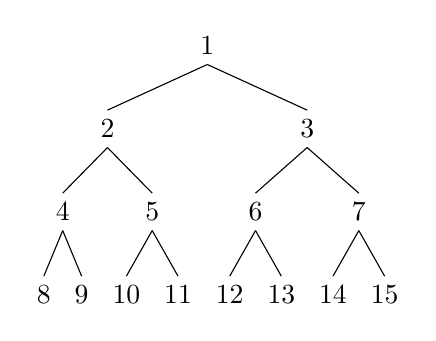
\begin{tikzpicture}
\Tree [.1 [.2 [.4 [.8 ] [.9 ] ] [.5 [.10 ] [.11 ] ] ] [.3 [.6 [.12 ] [.13 ] ] [.7 [.14 ] [.15 ] ] ] ]
\end{tikzpicture}

    Then an adjacency-list representation of a complete binary tree can be represented as such:
    

    $\fbox{1}\rightarrow\fbox{2}\rightarrow\fbox{3}$
    
    $\fbox{2}\rightarrow\fbox{4}\rightarrow\fbox{5}$
    
    $\fbox{3}\rightarrow\fbox{6}\rightarrow\fbox{7}$
    
    $\fbox{4}\rightarrow\fbox{8}\rightarrow\fbox{9}$
    
    $\fbox{5}\rightarrow\fbox{10}\rightarrow\fbox{11}$
    
    $\fbox{6}\rightarrow\fbox{12}\rightarrow\fbox{13}$
    
    $\fbox{7}\rightarrow\fbox{14}\rightarrow\fbox{15}$
    
    $\fbox{8}\rightarrow\fbox{$\emptyset$}$
    
    $\fbox{9}\rightarrow\fbox{$\emptyset$}$
    
    $\fbox{10}\rightarrow\fbox{$\emptyset$}$
    
    $\fbox{11}\rightarrow\fbox{$\emptyset$}$
    
    $\fbox{12}\rightarrow\fbox{$\emptyset$}$
    
    $\fbox{13}\rightarrow\fbox{$\emptyset$}$
    
    $\fbox{14}\rightarrow\fbox{$\emptyset$}$
    
    $\fbox{15}\rightarrow\fbox{$\emptyset$}$

The adjacency matrix representation is on the following page. 


\begin{table}[H]
\begin{tabular}{llllllllllllllll}
\hline
AdjM & 1 & 2 & 3 & 4 & 5 & 6 & 7 & 8 & 9 & 10 & 11 & 12 & 13 & 14 & 15 \\ \hline
1    & 0 & 1 & 1 & 0 & 0 & 0 & 0 & 0 & 0 & 0  & 0  & 0  & 0  & 0  & 0  \\
2    & 0 & 0 & 0 & 1 & 1 & 0 & 0 & 0 & 0 & 0  & 0  & 0  & 0  & 0  & 0  \\
3    & 0 & 0 & 0 & 0 & 0 & 1 & 1 & 0 & 0 & 0  & 0  & 0  & 0  & 0  & 0  \\
4    & 0 & 0 & 0 & 0 & 0 & 0 & 0 & 1 & 1 & 0  & 0  & 0  & 0  & 0  & 0  \\
5    & 0 & 0 & 0 & 0 & 0 & 0 & 0 & 0 & 0 & 1  & 1  & 0  & 0  & 0  & 0  \\
6    & 0 & 0 & 0 & 0 & 0 & 0 & 0 & 0 & 0 & 0  & 0  & 1  & 1  & 0  & 0  \\
7    & 0 & 0 & 0 & 0 & 0 & 0 & 0 & 0 & 0 & 0  & 0  & 0  & 0  & 1  & 1  \\
8    & 0 & 0 & 0 & 0 & 0 & 0 & 0 & 0 & 0 & 0  & 0  & 0  & 0  & 0  & 0  \\
9    & 0 & 0 & 0 & 0 & 0 & 0 & 0 & 0 & 0 & 0  & 0  & 0  & 0  & 0  & 0  \\
10   & 0 & 0 & 0 & 0 & 0 & 0 & 0 & 0 & 0 & 0  & 0  & 0  & 0  & 0  & 0  \\
11   & 0 & 0 & 0 & 0 & 0 & 0 & 0 & 0 & 0 & 0  & 0  & 0  & 0  & 0  & 0  \\
12   & 0 & 0 & 0 & 0 & 0 & 0 & 0 & 0 & 0 & 0  & 0  & 0  & 0  & 0  & 0  \\
13   & 0 & 0 & 0 & 0 & 0 & 0 & 0 & 0 & 0 & 0  & 0  & 0  & 0  & 0  & 0  \\
14   & 0 & 0 & 0 & 0 & 0 & 0 & 0 & 0 & 0 & 0  & 0  & 0  & 0  & 0  & 0  \\
15   & 0 & 0 & 0 & 0 & 0 & 0 & 0 & 0 & 0 & 0  & 0  & 0  & 0  & 0  & 0  \\ \hline
\end{tabular}

\end{table}

\end{solutionorbox}



\pagebreak
\newpage

%%%%%%%%%%%%%%%%%%%%%%%%%%%%%%%%%%%%%%%%%%%%%%%%%%%%%%%%%%%%%%%%%%
% Question
%%%%%%%%%%%%%%%%%%%%%%%%%%%%%%%%%%%%%%%%%%%%%%%%%%%%%%%%%%%%%%%%%%
\question[10]
The \textbf{\textit{incidence matrix}} of a directed graph $G=(V,E)$ with no self-loops is a $\abs{V} \times \abs{E}$ matrix $B = (b_{ij})$ such that
$$b_{ij} = \begin{cases}
	-1 & \text{if edge }j\text{ leaves vertex }i\text{,}\\
	1  & \text{if edge }j\text{ enters vertex }i\text{,}\\
	0  & \text{otherwise}
\end{cases}
$$

Describe what the entries of the matrix product $BB^T$ represent, where $B^T$ is the transpose of $B$.
\begin{solutionorbox}

    Let 
	Place answer here.
\end{solutionorbox}

\newpage


%%%%%%%%%%%%%%%%%%%%%%%%%%%%%%%%%%%%%%%%%%%%%%%%%%%%%%%%%%%%%%%%%%
% Question
%%%%%%%%%%%%%%%%%%%%%%%%%%%%%%%%%%%%%%%%%%%%%%%%%%%%%%%%%%%%%%%%%%
\question[10]
The BFS algorithm presented in class uses a queue as the data structure for storing discovered vertices.  Explain what would happen if you change the data structures to use a stack instead of a queue.  Use the graph example presented in lecture to demonstrate your solution.   
\begin{solutionorbox}
	Place answer here.
\end{solutionorbox}
	
\newpage



%%%%%%%%%%%%%%%%%%%%%%%%%%%%%%%%%%%%%%%%%%%%%%%%%%%%%%%%%%%%%%%%%%%
%% Question
%%%%%%%%%%%%%%%%%%%%%%%%%%%%%%%%%%%%%%%%%%%%%%%%%%%%%%%%%%%%%%%%%%%
%\question[10]
%Rewrite the procedure \proc{DFS}, using a stack to eliminate recursion.
%\begin{solutionorbox}
%	Place answer here.
%\end{solutionorbox}
%
%\newpage
%
%
%%%%%%%%%%%%%%%%%%%%%%%%%%%%%%%%%%%%%%%%%%%%%%%%%%%%%%%%%%%%%%%%%%
% Question
%%%%%%%%%%%%%%%%%%%%%%%%%%%%%%%%%%%%%%%%%%%%%%%%%%%%%%%%%%%%%%%%%%
\question[10]
Trace through the $\proc{Topological-Sort}$ algorithm and show the ordering of vertices produced on the following DAG.  Assume your \proc{DFS} algorithm processes the nodes in alphabetical order and the edges for each node in the adjacency list are also listed in alphabetical order.\\
\begin{center}
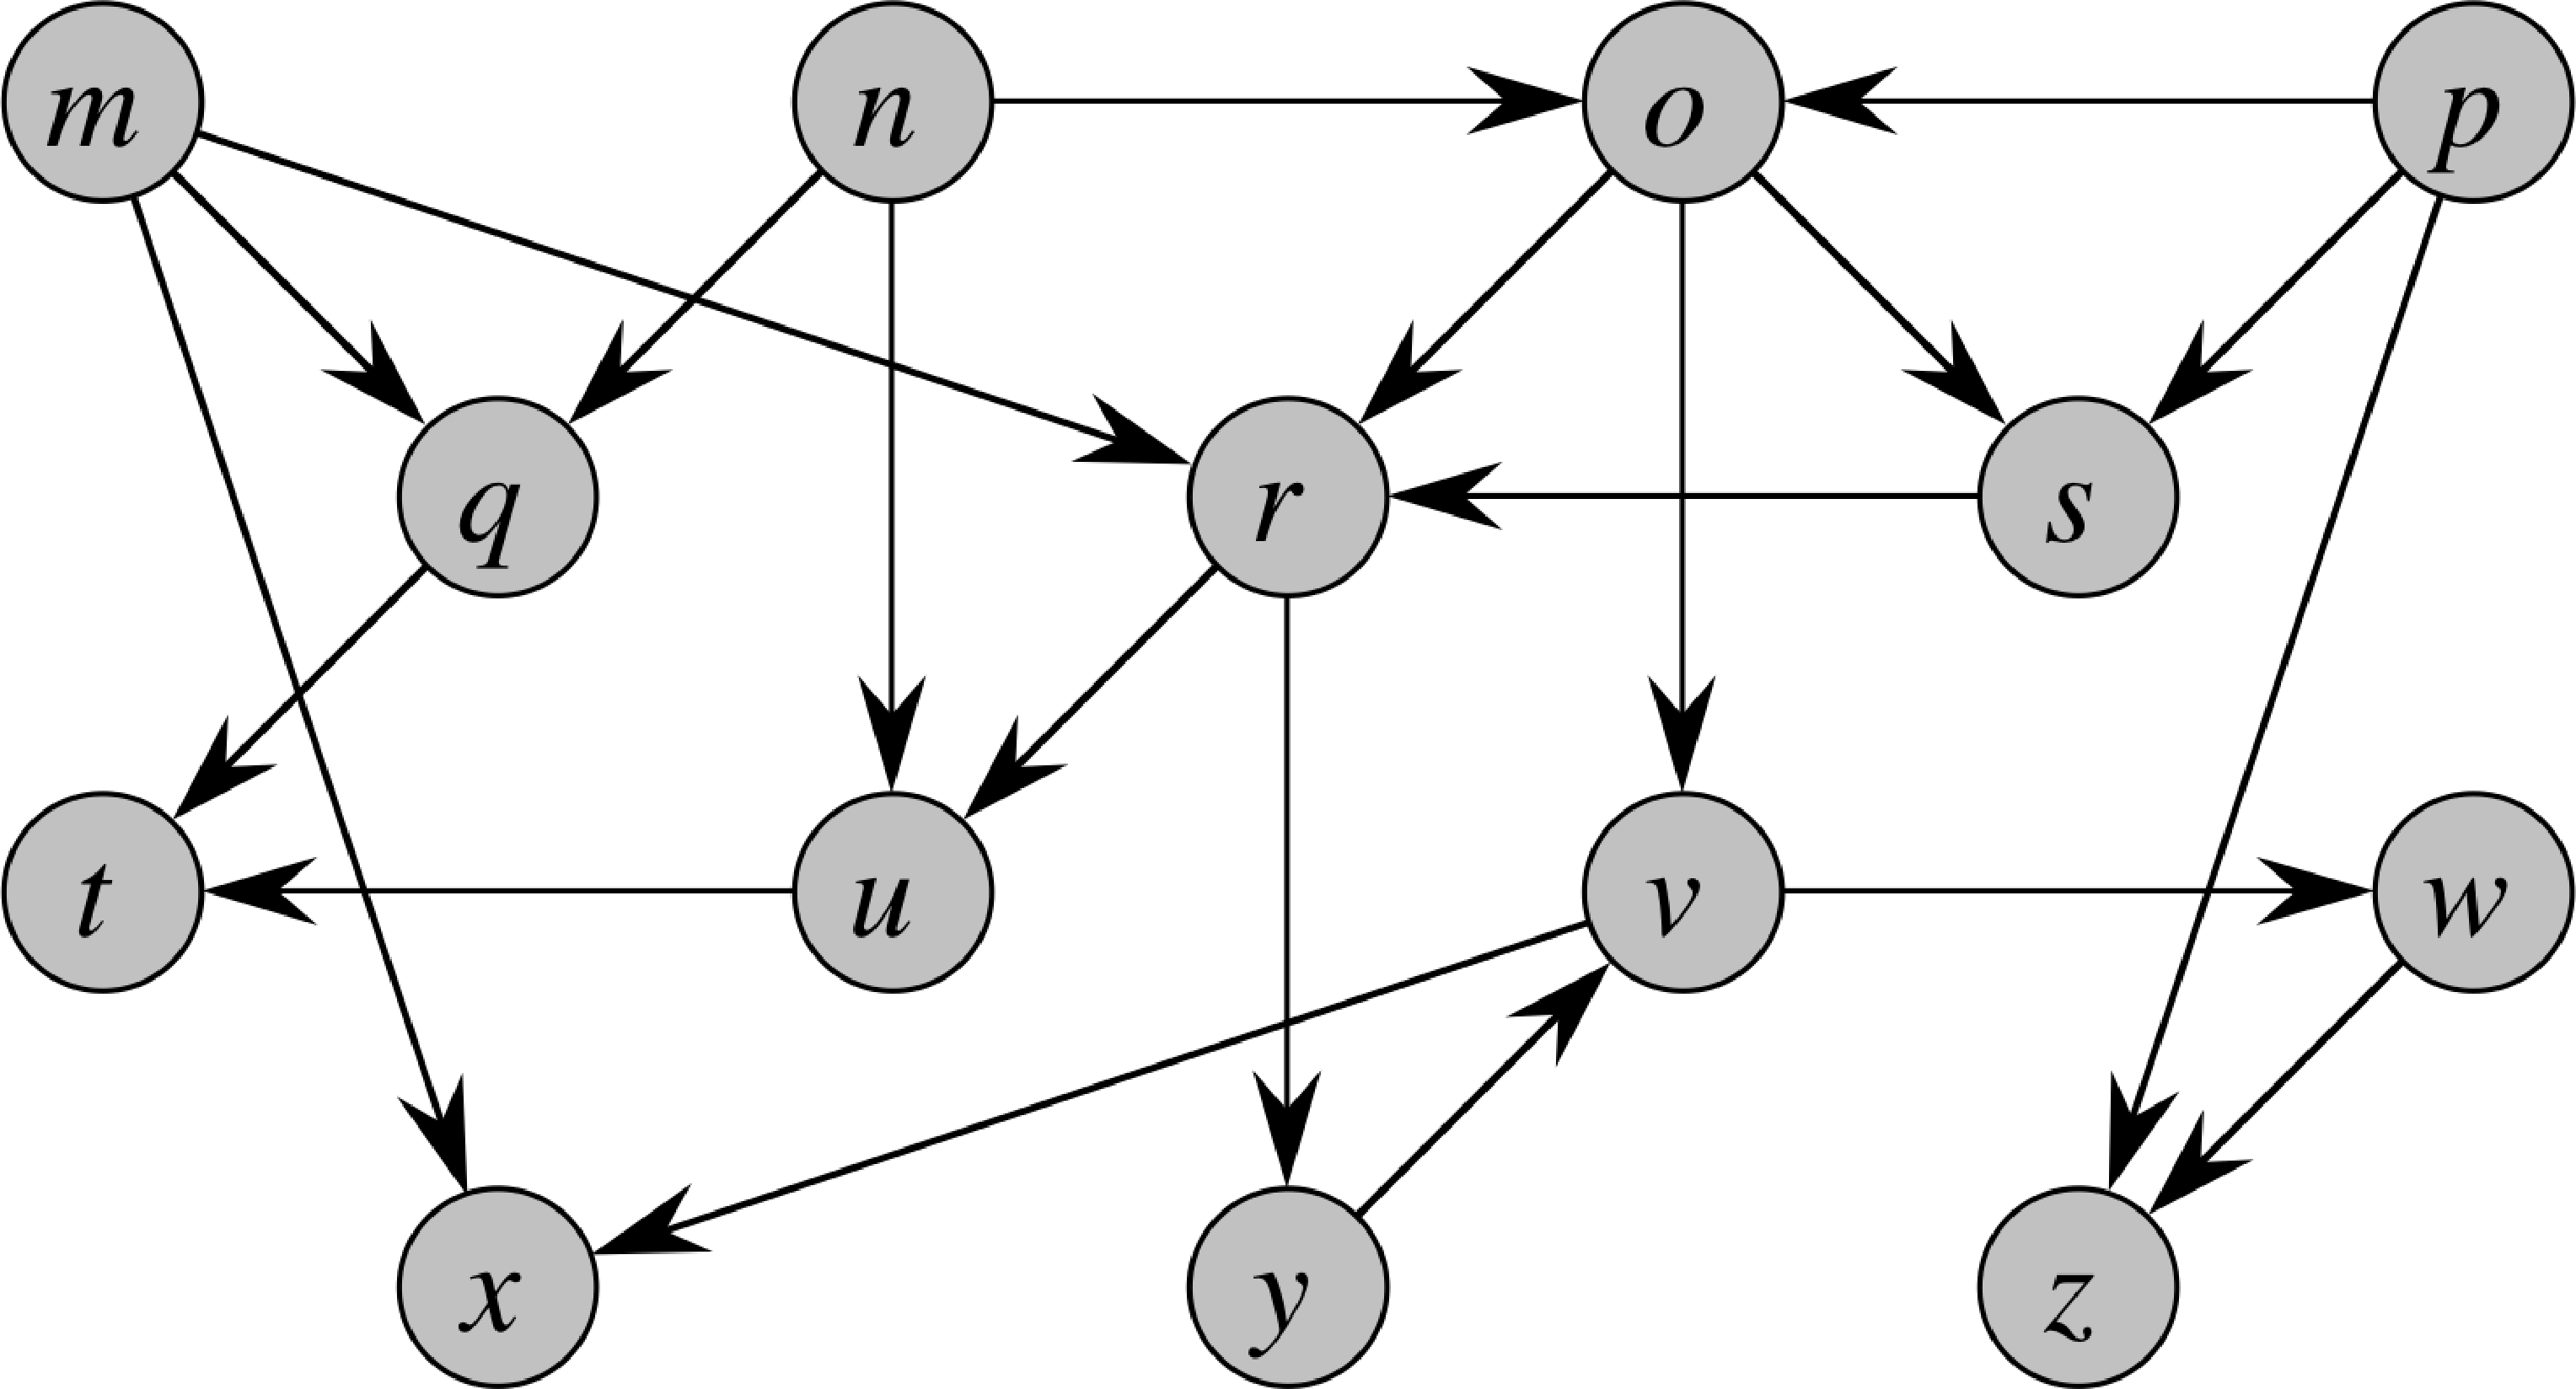
\includegraphics[scale=0.10]{Fig_05a.pdf}
\end{center}  

\begin{solutionorbox}
	Place answer here.
	One possible topological sort:
	
	Since we process nodes in alphabetical order, we will start at node m . There is no nodes we can travel to We will now mark m as visited (mark as explored).
	
	We move on to node n and mark as visited. We cannot go onto o or u just yet but we can visit q, so we mark it as encountered. We cannot visit any nodes from node q so we mark it as explored. 
	
	Move on to node o. Cannot move to any node yet so mark as explored. (mark x as visited)
	
	Move on to node p. (mark as visited). Move to node s, since you can. You can move onto node r as well. From r, we are looking in alphabetical order. u is on the adjecency list of u and we can visit it, so we will. From u, we can visit t. Back to node r, we will now visit node y. From y we will visit node v. From v we will go to w (alphabetical order.) from W we will go to z. From v we will finally go to x. 

	
	
	
	
	$\proc{Topological-Sort} = \left< m, n, q, o, p, s, r, u, t, y , v, w, z, x \right>$
	
	 
\end{solutionorbox}

\newpage


%%%%%%%%%%%%%%%%%%%%%%%%%%%%%%%%%%%%%%%%%%%%%%%%%%%%%%%%%%%%%%%%%%
%%%%%%%%%%%%%%%%%%%%%%%%%%%%%%%%%%%%%%%%%%%%%%%%%%%%%%%%%%%%%%%%%%
\end{questions}
\end{document}
